\documentclass[aspectratio=169, 10pt]{beamer}

%% ── Packages ──────────────────────────────────────────────────────────────
\usepackage[T1]{fontenc}
\usepackage{lmodern}
\usepackage{amsmath, amssymb}
\usepackage{booktabs}
\usepackage{graphicx}
\usepackage{tikz}
\usepackage{pgfplots}
\pgfplotsset{compat=1.18}
\hyphenpenalty=10000
\exhyphenpenalty=10000

%% ── Colour palette ────────────────────────────────────────────────────────
\definecolor{pnavy}{RGB}{15, 32, 67}
\definecolor{pblue}{RGB}{41, 98, 163}
\definecolor{plblue}{RGB}{120, 172, 220}
\definecolor{pred}{RGB}{200, 65, 55}
\definecolor{pgray}{RGB}{100, 105, 115}
\definecolor{plgray}{RGB}{242, 244, 247}
\definecolor{pgreen}{RGB}{50, 150, 100}

%% ── Base theme ────────────────────────────────────────────────────────────
\usetheme{default}
\setbeamertemplate{navigation symbols}{}
\setbeamercolor{background canvas}{bg=white}

%% ── Frame title ───────────────────────────────────────────────────────────
\setbeamercolor{frametitle}{fg=white, bg=pnavy}
\setbeamerfont{frametitle}{size=\small, series=\bfseries}
\setbeamertemplate{frametitle}{%
  \begin{beamercolorbox}[wd=\paperwidth, ht=2.6ex, dp=1.3ex, leftskip=1.5em]{frametitle}%
    \usebeamerfont{frametitle}\insertframetitle%
    \ifx\insertframesubtitle\empty\else
      \hspace{0.7em}{\scriptsize\textcolor{plblue}{\insertframesubtitle}}%
    \fi
  \end{beamercolorbox}%
  {\color{pblue}\hrule height 2pt}%
}

%% ── Footer ────────────────────────────────────────────────────────────────
\setbeamertemplate{footline}{%
  \hbox{%
    \begin{beamercolorbox}[wd=0.55\paperwidth, ht=2ex, dp=1.2ex, leftskip=1.5em]{author in head/foot}%
      \textcolor{pgray}{\tiny\insertshortauthor\ $\cdot$\ \insertshortinstitute}%
    \end{beamercolorbox}%
    \begin{beamercolorbox}[wd=0.3\paperwidth, ht=2ex, dp=1.2ex, center]{title in head/foot}%
      \textcolor{pgray}{\tiny\insertshorttitle}%
    \end{beamercolorbox}%
    \begin{beamercolorbox}[wd=0.15\paperwidth, ht=2ex, dp=1.2ex, rightskip=1.5em, right]{date in head/foot}%
      \textcolor{pgray}{\tiny\insertframenumber\,/\,\inserttotalframenumber}%
    \end{beamercolorbox}%
  }%
}

%% ── Bullets ───────────────────────────────────────────────────────────────
\setbeamercolor{itemize item}{fg=pblue}
\setbeamercolor{itemize subitem}{fg=plblue}
\setbeamertemplate{itemize item}{%
  \footnotesize\raisebox{0.15ex}{\textcolor{pblue}{$\blacktriangleright$}}}
\setbeamertemplate{itemize subitem}{%
  \scriptsize\raisebox{0.15ex}{\textcolor{plblue}{$\triangleright$}}}

%% ── Blocks ────────────────────────────────────────────────────────────────
\setbeamercolor{block title}{fg=white, bg=pblue}
\setbeamercolor{block body}{fg=black, bg=plgray}
\setbeamerfont{block title}{size=\small, series=\bfseries}
\setbeamercolor{alerted text}{fg=pred}
\setbeamerfont{alerted text}{series=\bfseries}

%% ── Title page ────────────────────────────────────────────────────────────
\setbeamerfont{title}{size=\Large, series=\bfseries}
\setbeamercolor{title}{fg=white}

\setbeamertemplate{title page}{%
  \begin{tikzpicture}[remember picture, overlay]
    %% ── Background bands
    \fill[pnavy] (current page.north west)
      rectangle ([yshift=-0.62\paperheight]current page.north east);
    \fill[pblue] ([yshift=-0.62\paperheight]current page.north west)
      rectangle ([yshift=-0.645\paperheight]current page.north east);
    %% ── Title + subtitle centred in the navy band
    \node[anchor=center, text width=0.82\paperwidth, align=center]
      at ([yshift=-0.27\paperheight]current page.north) {%
        {\usebeamerfont{title}\textcolor{white}{\inserttitle}}\\[0.55em]
        {\small\textcolor{plblue}{\insertsubtitle}}%
      };
    %% ── Author block in the white area below the stripe
    \node[anchor=north west, text width=0.82\paperwidth, align=left]
      at ([xshift=0.09\paperwidth, yshift=-0.68\paperheight]current page.north west) {%
        {\small\textbf{\textcolor{pnavy}{Yvan Richard, Antoine Pittet, Arthur Glauser, Samuel Payne \& Alexandre Zaza}}}\\[0.35em]
        {\small\textcolor{pgray}{\insertinstitute}}\\[0.15em]
        {\small\textcolor{pgray}{\insertdate}}%
      };
  \end{tikzpicture}%
}

%% ── Section divider ───────────────────────────────────────────────────────
\AtBeginSection[]{%
  \begin{frame}[plain]
    \begin{tikzpicture}[remember picture, overlay]
      \fill[pnavy] (current page.south west) rectangle (current page.north east);
      \fill[pblue] ([yshift=-0.01\paperheight]current page.center)
        rectangle ([yshift=-0.025\paperheight]current page.center
          -| current page.east);
      \node[anchor=center, text width=0.72\paperwidth, align=center]
        at (current page.center) {%
          \textcolor{white}{\Large\bfseries\insertsectionhead}%
        };
      \node[anchor=south, yshift=1.5em] at (current page.south) {%
        \begin{minipage}{0.80\paperwidth}
          \centering
          \textcolor{plgray}{\small\insertshortauthor}\\[0.25em]
          \textcolor{plblue}{\scriptsize\insertshortinstitute\ $\cdot$\ \insertshorttitle}%
        \end{minipage}%
      };
    \end{tikzpicture}
  \end{frame}%
}

%% ── Metadata ──────────────────────────────────────────────────────────────
\title{How Attention Shapes the Trading Behavior of Retail Investors}
\subtitle{Interpreting Statistical Data from Behavioral Research}
\author[Y.\ Richard \& A.\ Pittet \& A.\ Glauser \& S.\ Payne \& A.\ Zaza]{Yvan Richard \and Antoine Pittet \and Arthur Glauser \and Samuel Payne \and Alexandre Zaza}
\institute[HSG]{University of St.\ Gallen}
\date{Spring Semester 2026}

%%%%%%%%%%%%%%%%%%%%%%%%%%%%%%%%%%%%%%%%%%%%%%%%%%%%%%%%%%%%%%%%%%%%%%%%%%%
\begin{document}
%%%%%%%%%%%%%%%%%%%%%%%%%%%%%%%%%%%%%%%%%%%%%%%%%%%%%%%%%%%%%%%%%%%%%%%%%%%

%% ── Title ─────────────────────────────────────────────────────────────────
\begin{frame}[plain]
  \titlepage
\end{frame}

%% ── Outline ───────────────────────────────────────────────────────────────
\begin{frame}{Outline}
  \tableofcontents
\end{frame}

%%──────────────────────────────────────────────────────────────────────────
\section{Introduction}
%%──────────────────────────────────────────────────────────────────────────

%% 1.1. Research Question
%%──────────────────────────────────────────────────────────────────────────
\begin{frame}{Why Study the Effect of Attention on Trading Behavior?}
  \begin{columns}[T]
    \begin{column}{0.53\textwidth}
      \textbf{The Search Problem for Retail Investors}
      \vspace{0.5em}
      \begin{itemize}
        \setlength\itemsep{0.5em}
        \item Retail investors face an asymmetric universe of stocks ($U = \{1, \dots, N\}$), depending on whether they are \emph{buying} or \emph{selling}.
        \item Due to short constraints, individual investors can only sell stocks they already hold: $\mid U_{sell} \mid \approx 5$.
        \item However, during a buying decision, they must search across \alert{thousands} of investable securities: $\mid U_{buy} \mid \approx 8,000$.
        \item Attention is a scarce resource and might play a crucial role in determining which stocks are purchased.
      \end{itemize}
    \end{column}
    \begin{column}{0.43\textwidth}
      \begin{block}{Research Question}
        How does attention affect the trading behavior of retail investors, particularly in
        the context of buying decisions where the choice set is large and complex? Does this effect
        differ depending on the type of signal (e.g., news, social media, Google Search) that captures investors' attention?
      \end{block}
    \end{column}
  \end{columns}
\end{frame}

%% 1.2. Literature Review
%% _________________________________________________________________________
\begin{frame}{Related Literature}
  \begin{columns}[T]
    \begin{column}{0.48\textwidth}
      \textbf{Attention Signals and Trading Behavior}
      \vspace{0.5em}
      \begin{itemize}
        \setlength\itemsep{0.5em}
        \item Barber and Odean (2008): \textit{All That Glitters: The Effect of Attention and News on the Buying Behavior of Individual and Institutional Investors.}
        \item Da, Engelberg, and Gao (2011): \textit{In Search of Attention.}
        \item Barber et al. (2022): \textit{Attention-Induced Trading and Returns: Evidence from Robinhood Users.}
      \end{itemize}
    \end{column}
    \begin{column}{0.48\textwidth}
      \textbf{Gaps in the Literature}
      \vspace{0.5em}
      \begin{itemize}
        \setlength\itemsep{0.5em}
        \item Most studies focus on population level effects, with limited insights into individual heterogeneity in attention and trading behavior.
        \item Limited understanding of how different types of attention signals (e.g., news vs.\ social media) differentially impact trading decisions.
        \item No causal evidence on the mechanisms through which attention influences trading behavior (i.e., no proper experimental design).
      \end{itemize}
    \end{column}
  \end{columns}
\end{frame}

%% 1.3. Hypotheses
%% _________________________________________________________________________
\begin{frame}{Hypotheses}
  \begin{columns}[T]
    \begin{column}{0.48\textwidth}
      \begin{itemize}
        \setlength\itemsep{1.0em}
        \item[\textbf{H1}] \textbf{Exposure Level:} High media exposure produces \alert{higher} buying intention than low exposure.
        \item[\textbf{H2}] \textbf{Media Channel:} The type of attention signal affects buying intention; Social Media $>$ News $>$ Google Search.
      \end{itemize}
    \end{column}
    \begin{column}{0.48\textwidth}
      \begin{itemize}
        \setlength\itemsep{1.0em}
        \item[\textbf{H3}] \textbf{Industry:} Buying intention differs across stock industry sectors.
        \item[\textbf{H4}] \textbf{Interactions:} The effect of one factor depends on the level of another — in particular, exposure amplifies the media channel effect.
      \end{itemize}
    \end{column}
  \end{columns}
\end{frame}

%%──────────────────────────────────────────────────────────────────────────
\section{Methodology, Data \& Design}
%%──────────────────────────────────────────────────────────────────────────

%% 2.1. Sample Overview
%% _________________________________________________________________________
\begin{frame}{Sample Overview}
  \begin{columns}[T]
    \begin{column}{0.42\textwidth}
      {\small\textbf{Dataset}}
      \vspace{0.3em}
      {\footnotesize
      \begin{itemize}
        \setlength\itemsep{0.25em}
        \item $N = 720$, balanced $3 \times 2 \times 2$ factorial design
        \item 12 cells, 60 obs.\ each; no missing values
        \item Buying intention: $M = 2.97$, $SD = 0.80$, $Mdn = 3$
      \end{itemize}
      }
      \vspace{0.4em}
      {\small\textbf{Group Sizes}}
      \vspace{0.2em}
      {\scriptsize
      \begin{tabular}{lc}
        \toprule
        \textbf{Group} & $N$ \\
        \midrule
        Google Search & 240 \\
        News & 240 \\
        Social Media & 240 \\
        \midrule
        High Exposure & 360 \\
        Low Exposure & 360 \\
        \midrule
        Industry A & 360 \\
        Industry B & 360 \\
        \bottomrule
      \end{tabular}
      }
    \end{column}
    \begin{column}{0.54\textwidth}
      \vspace{0.2em}
      \begin{center}
        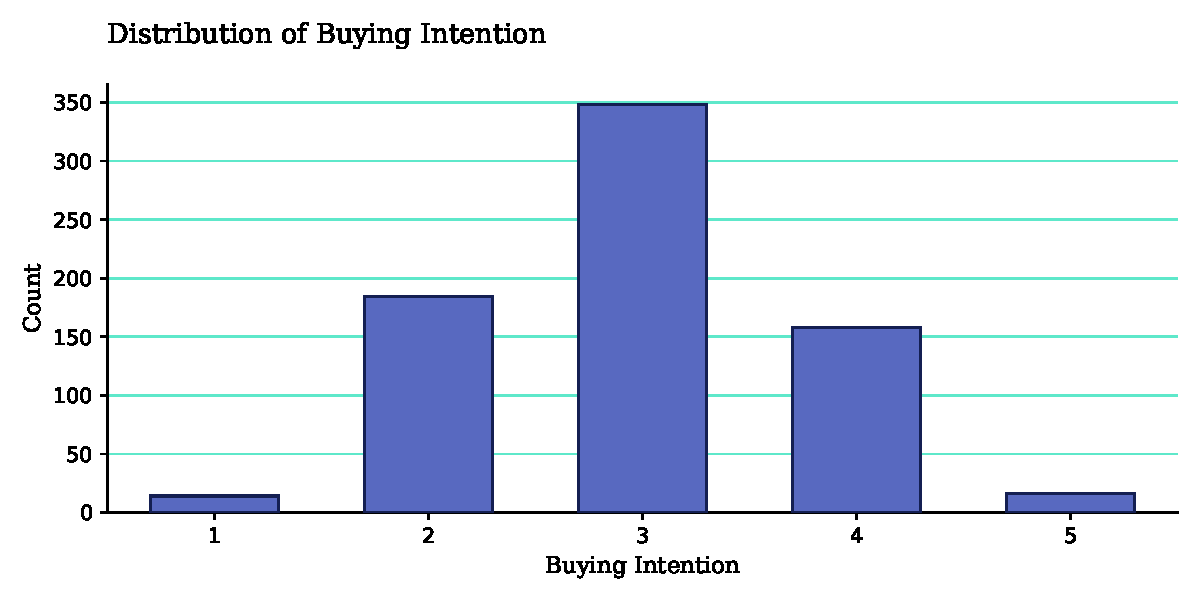
\includegraphics[width=\columnwidth]{../../../results/plots/buying_intention_distribution.pdf}
      \end{center}
      {\scriptsize\textcolor{pgray}{Most responses cluster at 3; scores of 1 and 5 occur rarely, indicating adequate central spread for group comparisons.}}
    \end{column}
  \end{columns}
\end{frame}

%% 2.2. Experimental Design
%% _________________________________________________________________________
\begin{frame}{Experimental Design}
  \begin{columns}[T]
    \begin{column}{0.46\textwidth}
      \textbf{Design}
      \vspace{0.4em}
      \begin{itemize}
        \setlength\itemsep{0.45em}
        \item Between-subjects $3 \times 2 \times 2$ factorial experiment
        \item 12 experimental conditions, 60 participants per cell
        \item Participants randomly assigned to exactly one condition
        \item Post-exposure survey: buying intention recorded immediately after the stimulus (in ideal conditions)
      \end{itemize}
    \end{column}
    \begin{column}{0.50\textwidth}
      \textbf{Variables}
      \vspace{0.4em}
      {\footnotesize
      \renewcommand{\arraystretch}{1.3}
      \begin{tabular}{p{2.1cm}p{0.65cm}p{2.7cm}}
        \toprule
        \textbf{Variable} & \textbf{Role} & \textbf{Levels} \\
        \midrule
        Media Attention & IV1 & Google Search, News, Social Media \\
        Exposure Level & IV2 & Low, High \\
        Industry & IV3 & Industry A, Industry B \\
        Buying Intention & DV & 1--5 ordinal scale \\
        \bottomrule
      \end{tabular}
      }
    \end{column}
  \end{columns}
\end{frame}

%% 2.3. Materials \& Tools
%% _________________________________________________________________________
\begin{frame}{Materials \& Tools}
  \begin{columns}[T]
    \begin{column}{0.50\textwidth}
      \textbf{Measurement Instrument}
      \vspace{0.4em}
      \begin{itemize}
        \setlength\itemsep{0.45em}
        \item Structured questionnaire with channel-specific experimental stimuli:
          \begin{itemize}
            \setlength\itemsep{0.2em}
            \item Search-result interface (Google Search)
            \item Formatted news article (News)
            \item Social-media feed post (Social Media)
          \end{itemize}
        \item Each stimulus presented at a low or high exposure intensity
        \item Buying intention measured on a 5-point Likert-type scale:\\[0.2em]
          {\scriptsize\textit{1 = very unlikely} \quad $\cdots$ \quad \textit{5 = very likely}}
      \end{itemize}
    \end{column}
    \begin{column}{0.46\textwidth}
      \textbf{Statistical Software}
      \vspace{0.4em}
      \begin{itemize}
        \setlength\itemsep{0.45em}
        \item \textbf{Jamovi}: preliminary tests for fast iteration
        \item \textbf{Python 3.13}: reproducible analysis pipeline
        \item \texttt{pandas / numpy}: data manipulation
        \item \texttt{statsmodels}: ANOVA, OLS regression, Tukey's HSD
        \item \texttt{scipy}: Shapiro-Wilk normality test
        \item \texttt{seaborn / matplotlib}: visualisations
      \end{itemize}
    \end{column}
  \end{columns}
\end{frame}

%% 2.3b. Exploratory Analysis
%% _________________________________________________________________________
\begin{frame}{Exploratory Analysis}
  \begin{center}
    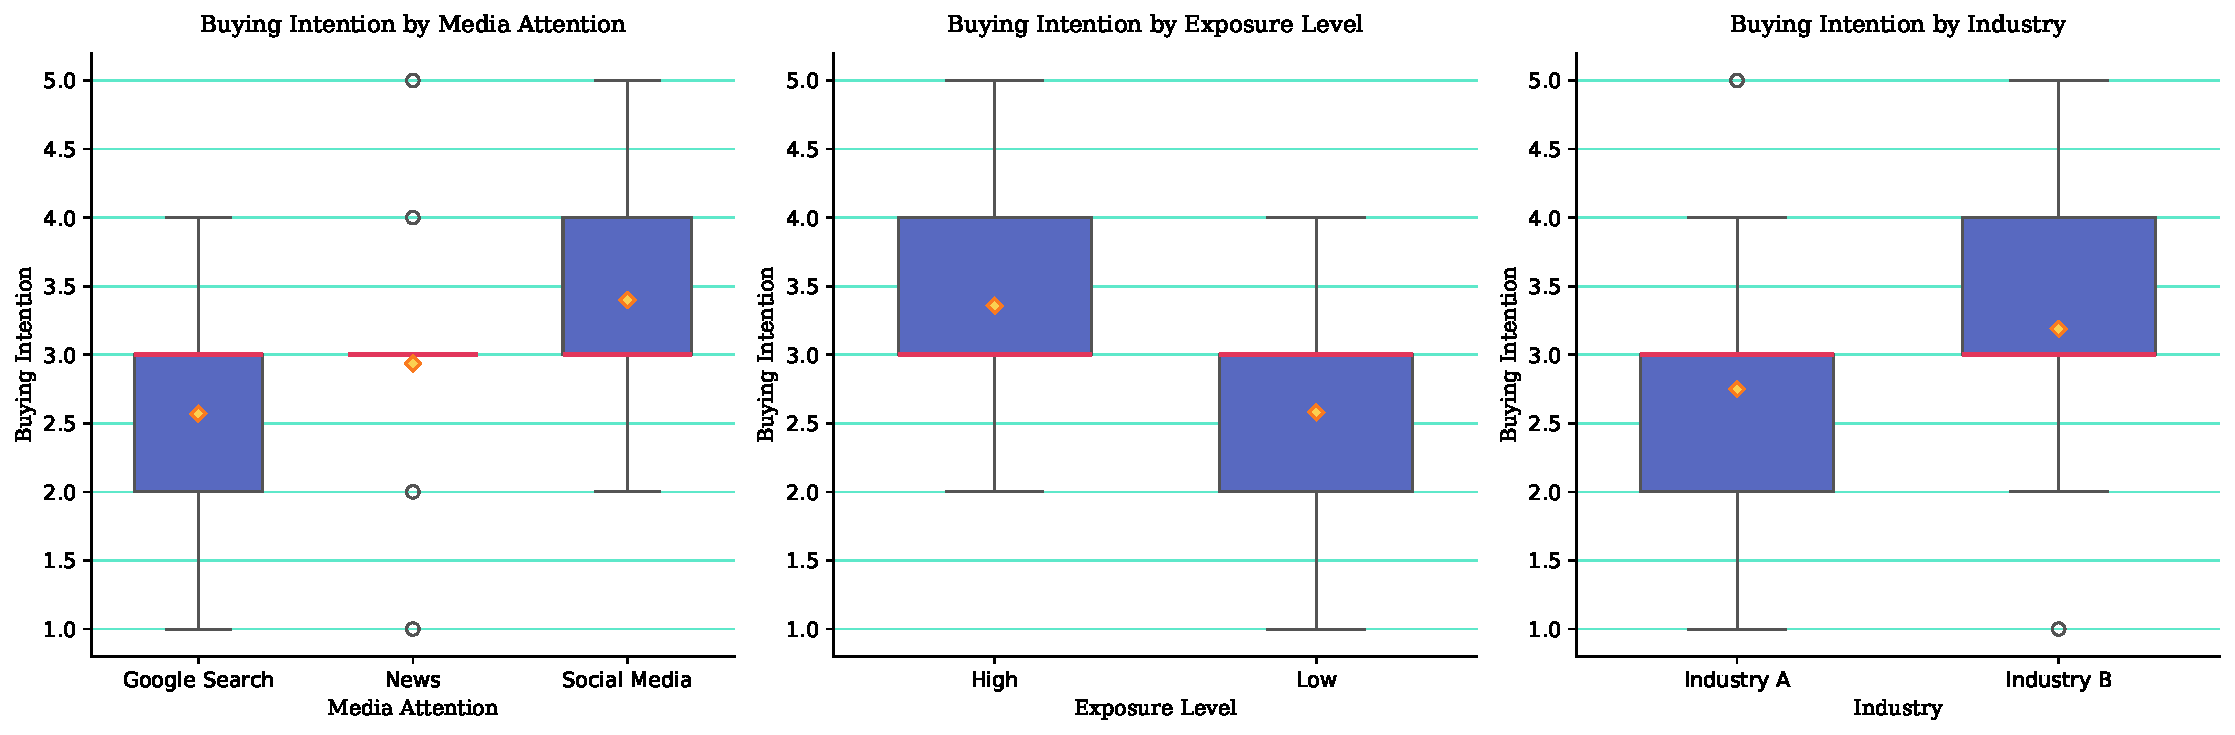
\includegraphics[width=0.96\textwidth]{../../../results/plots/bivariate_analysis.pdf}
  \end{center}
  \vspace{-0.4em}
  {\footnotesize
  \begin{itemize}
    \setlength\itemsep{0.15em}
    \item \textbf{Media channel:} Social Media shows the highest central tendency and widest upward spread; Google Search the lowest.
    \item \textbf{Exposure level:} High exposure shifts the entire distribution upward relative to Low.
    \item \textbf{Industry:} Participants display stronger buying intention for Industry B compared to Industry A.
    \item \textcolor{pgray}{\textit{These are preliminary visual patterns; formal statistical tests are required to confirm significance.}}
  \end{itemize}
  \vspace{0.2em}
  {\scriptsize\textcolor{pgray}{\textit{Note:} \textcolor{pred}{$\rule{1em}{1.5pt}$} red bar = median \quad \textcolor{yellow!70!orange}{$\blacklozenge$} yellow diamond = mean.}}
  }
\end{frame}

%% 2.4. Statistical Analysis
%% _________________________________________________________________________
\begin{frame}{Statistical Analysis}
  \begin{columns}[T]
    \begin{column}{0.50\textwidth}
      \textbf{Three-Way ANOVA}
      \vspace{0.4em}
      \begin{itemize}
        \setlength\itemsep{1em}
        \item Type II sums of squares — robust to unbalanced designs
        \item Tests all main effects and interactions simultaneously
        \item Partial effect size: \\[0.8em]
          $\displaystyle \eta^2_p = 
          \frac{SS_{\text{effect}}}{SS_{\text{effect}} + SS_{\text{residual}}}$
        \item Post-hoc pairwise comparisons: Tukey's HSD ($\text{FWER} = .05$)
      \end{itemize}
    \end{column}
    \begin{column}{0.46\textwidth}
      \textbf{OLS Regression}
      \vspace{0.4em}
      \begin{itemize}
        \setlength\itemsep{0.35em}
        \item Model 1: main effects only
        \item Model 2: full model with all two-way and three-way interactions
        \item HC3 heteroskedasticity-robust standard errors
        \item Model comparison via adjusted $R^2$ and AIC (Akaike Information Criterion)
      \end{itemize}
      \vspace{0.5em}
      \textbf{Diagnostics}
      \vspace{0.3em}
      \begin{itemize}
        \setlength\itemsep{0.35em}
        \item Shapiro-Wilk test for residual normality
        \item Breusch-Pagan test for heteroskedasticity
        \item Q-Q plot inspection
      \end{itemize}
    \end{column}
  \end{columns}
\end{frame}

%%──────────────────────────────────────────────────────────────────────────
\section{Empirical Results}
%%──────────────────────────────────────────────────────────────────────────

%% 3.1. ANOVA Results
%% _________________________________________________________________________
\begin{frame}{ANOVA Results}
  \framesubtitle{Three-way ANOVA, Type II SS — $N = 720$, $df_{\text{residual}} = 708$}
  \begin{columns}[T]
    \begin{column}{0.50\textwidth}
      {\scriptsize
      \renewcommand{\arraystretch}{1.10}
      \begin{tabular}{lrrrl}
        \toprule
        \textbf{Effect} & \textbf{df} & \textbf{F} & \textbf{p} & $\boldsymbol{\eta^2_p}$ \\
        \midrule
        \multicolumn{5}{l}{\textit{Main Effects}} \\
        \quad Media Attention    & 2 & \textbf{129.04} & $<\!.001$ & \textbf{.267} \\
        \quad Exposure Level     & 1 & \textbf{339.12} & $<\!.001$ & \textbf{.324} \\
        \quad Industry           & 1 & \textbf{107.98} & $<\!.001$ & \textbf{.132} \\
        \midrule
        \multicolumn{5}{l}{\textit{Two-Way Interactions}} \\
        \quad Media $\times$ Exposure  & 2 & \textbf{10.20} & $<\!.001$ & \textbf{.028} \\
        \quad Media $\times$ Industry  & 2 & 0.13 & $.875$ & .000 \\
        \quad Exposure $\times$ Industry & 1 & 0.28 & $.599$ & .000 \\
        \midrule
        \multicolumn{5}{l}{\textit{Three-Way Interaction}} \\
        \quad Media $\times$ Exp.\ $\times$ Ind. & 2 & 1.30 & $.273$ & .004 \\
        \midrule
        \quad Residual           & 708 & & & \\
        \bottomrule
      \end{tabular}
      }
      \vspace{0.2em}
      {\tiny\textcolor{pgray}{Bold = statistically significant ($p < .05$).}}
    \end{column}
    \begin{column}{0.46\textwidth}
      \begin{center}
        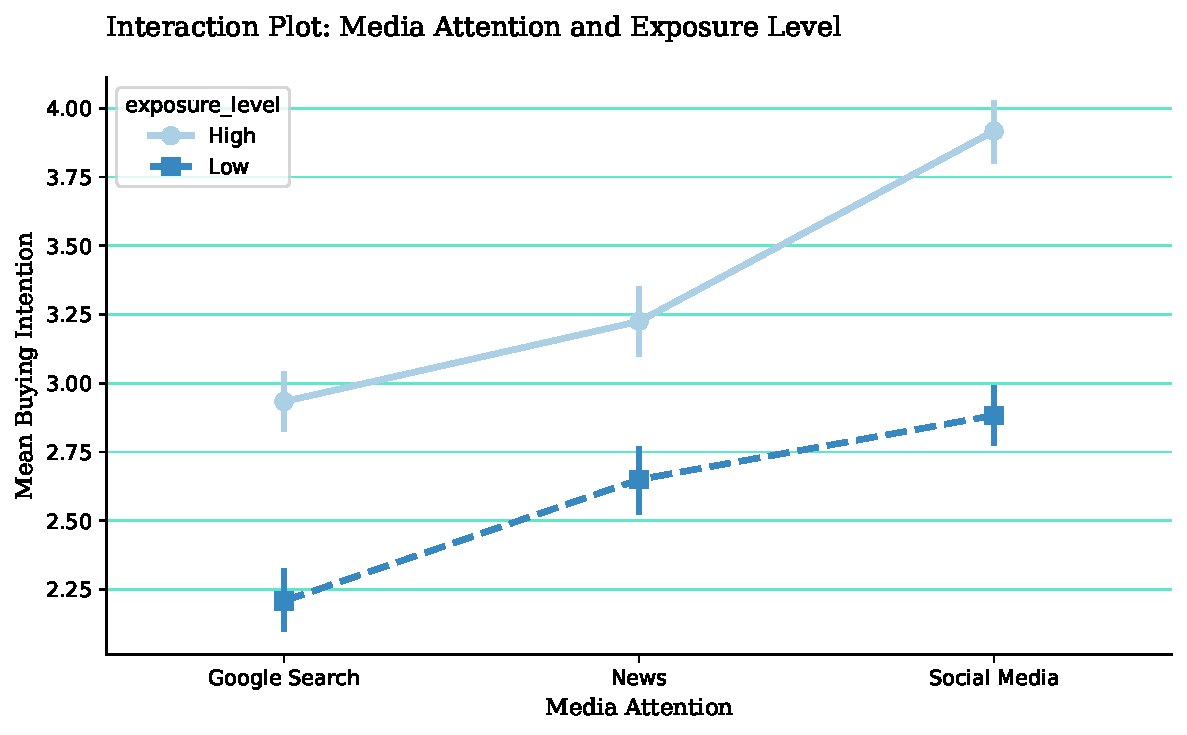
\includegraphics[width=\columnwidth]{../../../results/plots/interaction_plot.pdf}
      \end{center}
      {\scriptsize\textcolor{pgray}{High exposure raises buying intention most strongly for Social Media — supporting H4.}}
    \end{column}
  \end{columns}
\end{frame}

%% 3.1b. Model Assumptions
%% _________________________________________________________________________
\begin{frame}{Model Assumptions}
  \begin{columns}[T]
    \begin{column}{0.49\textwidth}
      \centering
      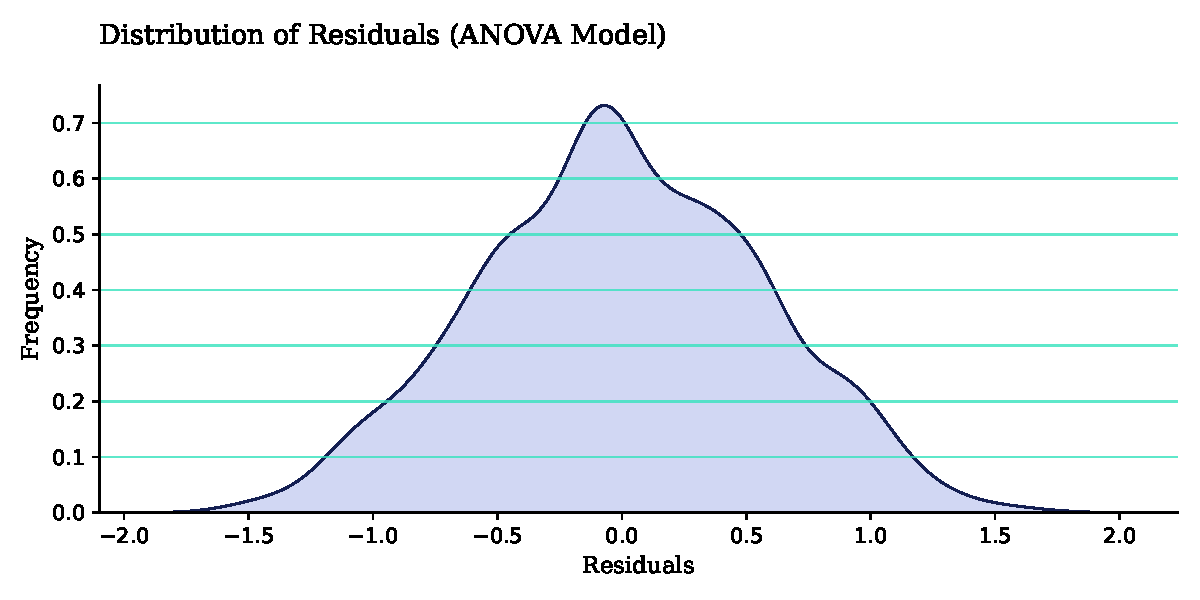
\includegraphics[width=\columnwidth]{../../../results/plots/residuals_distribution.pdf}
    \end{column}
    \begin{column}{0.49\textwidth}
      \centering
      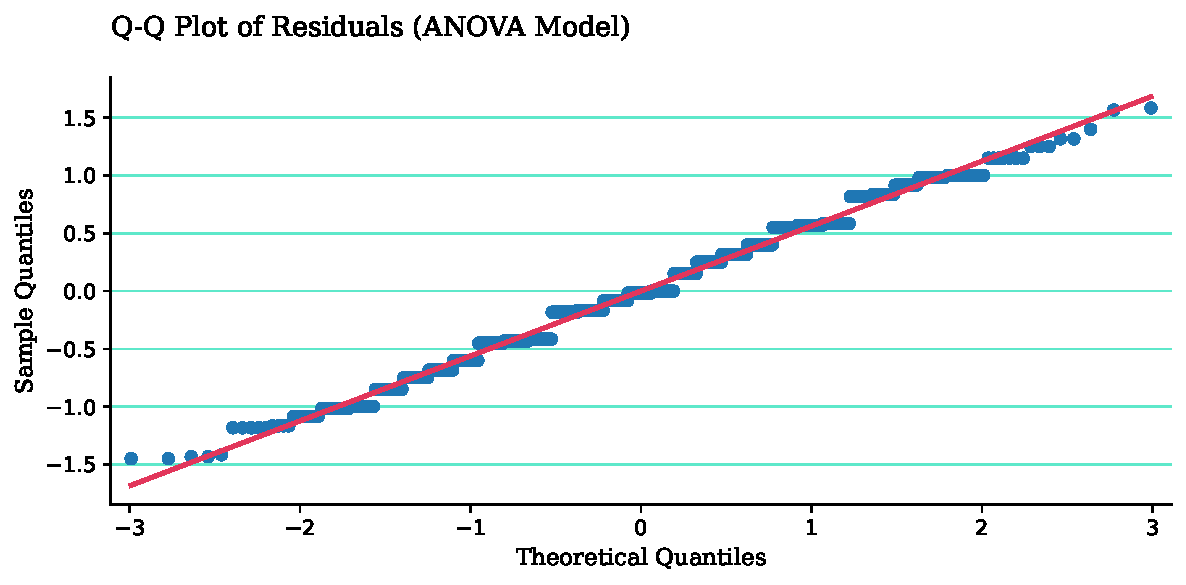
\includegraphics[width=\columnwidth]{../../../results/plots/residuals_qqplot.pdf}
    \end{column}
  \end{columns}
  \vspace{0.15em}
  \begin{columns}[T]
    \begin{column}{0.49\textwidth}
      {\footnotesize\textbf{Normality}}
      \vspace{0.1em}
      {\footnotesize
      \begin{itemize}
        \setlength\itemsep{0.15em}
        \item \textcolor{pred}{Shapiro-Wilk: $W = 0.990$, $p < .001$}
        \item Sensitive at large $N$ justifies this result; in fact, minor departure only! Visual inspection is key.
        \item Mid-range residuals closely follow the reference line
      \end{itemize}
      }
    \end{column}
    \begin{column}{0.49\textwidth}
      {\footnotesize\textbf{Homoskedasticity}}
      \vspace{0.1em}
      {\footnotesize
      \begin{itemize}
        \setlength\itemsep{0.15em}
        \item \textcolor{pgreen}{Breusch-Pagan: $LM = 4.50$, $p = .953$}
        \item No heteroskedasticity detected
        \item HC3 robust SEs confirm all main effects
      \end{itemize}
      }
    \end{column}
  \end{columns}
  \vspace{1em}
  {\scriptsize\textcolor{pgray}{$\Rightarrow$ Residuals are adequate for inference; main conclusions are robust.}}
\end{frame}

%% 3.2. Regression Results
%% _________________________________________________________________________
\begin{frame}{Regression Results}
  \framesubtitle{OLS — reference group: Google Search, High Exposure, Industry A}
  \begin{columns}[T]
    \begin{column}{0.56\textwidth}
      {\scriptsize
      \renewcommand{\arraystretch}{1.05}
      \begin{tabular}{lcc}
        \toprule
        & \textbf{Model 1} & \textbf{Model 2} \\
        & \textit{Main effects} & \textit{Full interaction} \\
        \midrule
        Intercept
          & $2.74^{***}$ & $2.68^{***}$ \\
          & \textcolor{pgray}{$(0.048)$} & \textcolor{pgray}{$(0.073)$} \\[0.3em]
        News (vs.\ Google Search)
          & $0.37^{***}$ & $0.33^{**}$ \\
          & \textcolor{pgray}{$(0.052)$} & \textcolor{pgray}{$(0.104)$} \\[0.3em]
        Social Media (vs.\ Google Search)
          & $0.83^{***}$ & $1.07^{***}$ \\
          & \textcolor{pgray}{$(0.052)$} & \textcolor{pgray}{$(0.104)$} \\[0.3em]
        Low Exposure (vs.\ High)
          & $-0.78^{***}$ & $-0.68^{***}$ \\
          & \textcolor{pgray}{$(0.043)$} & \textcolor{pgray}{$(0.104)$} \\[0.3em]
        Industry B (vs.\ A)
          & $0.44^{***}$ & $0.50^{***}$ \\
          & \textcolor{pgray}{$(0.043)$} & \textcolor{pgray}{$(0.104)$} \\[0.3em]
        Social Media $\times$ Low
          & $-$ & $-0.47^{**}$ \\
          & & \textcolor{pgray}{$(0.146)$} \\
        \midrule
        $R^2$ & $.491$ & $.507$ \\
        Adj.\ $R^2$ & $.488$ & $.500$ \\
        AIC & $1246.8$ & $1237.2$ \\
        \bottomrule
      \end{tabular}
      }\\[0.3em]
      {\tiny\textcolor{pgray}{$^{***}p<.001$,\ $^{**}p<.01$. Standard errors in parentheses. Only significant interaction term shown in Model 2.}}
    \end{column}
    \begin{column}{0.40\textwidth}
      \textbf{Key Takeaways}
      \vspace{0.4em}
      \begin{itemize}
        \setlength\itemsep{0.45em}
        \item All main effects significant at $p < .001$
        \item Social Media adds $+0.83$ pts over Google Search; high exposure adds $+0.78$ pts over low
        \item Industry B adds $+0.44$ pts over Industry A
        \item Full model preferred (AIC $1237 < 1247$)
        \item Social Media $\times$ Low: $-0.47^{**}$ — the channel's advantage shrinks sharply at low exposure
      \end{itemize}
    \end{column}
  \end{columns}
\end{frame}

%%──────────────────────────────────────────────────────────────────────────
\section{Interpretation \& Discussion}
%%──────────────────────────────────────────────────────────────────────────

%% 4.1. Finding 1
%% _________________________________________________________________________
\begin{frame}{Finding 1: Visibility Is the Primary Driver}
  \begin{columns}[T]
    \begin{column}{0.54\textwidth}
      \textbf{Exposure Level — Strongest Effect ($\eta^2_p = .324$)}
      \vspace{0.4em}
      \begin{itemize}
        \setlength\itemsep{0.45em}
        \item $F(1, 708) = 339.12$, $p < .001$
        \item High: $\bar{x} = 3.36$ vs.\ Low: $\bar{x} = 2.58$ $\;(\Delta = +0.78)$
        \item Tukey's HSD: $p < .001$; OLS: $+0.78^{***}$
      \end{itemize}
      \vspace{0.6em}
      \textbf{Industry ($\eta^2_p = .132$)}
      \vspace{0.4em}
      \begin{itemize}
        \setlength\itemsep{0.45em}
        \item $F(1, 708) = 107.98$, $p < .001$
        \item Industry B: $\bar{x} = 3.19$ vs.\ A: $\bar{x} = 2.75$ $\;(\Delta = +0.44)$
        \item Tukey's HSD: $p < .001$; OLS: $+0.44^{***}$
      \end{itemize}
    \end{column}
    \begin{column}{0.42\textwidth}
      \begin{block}{Interpretation}
        Consistent with the \textbf{limited attention framework}: higher visibility lowers the effective search cost and activates the \emph{familiarity heuristic}. When a stock enters an investor's awareness, mere exposure raises perceived relevance (independently of underlying fundamentals).

        \vspace{0.5em}
        Industry sector likely proxies for perceived risk and growth profile, creating heterogeneous baseline attractiveness across experimental conditions.
      \end{block}
    \end{column}
  \end{columns}
\end{frame}

%% 4.2. Finding 2
%% _________________________________________________________________________
\begin{frame}{Finding 2: Social Media Generates the Strongest Signal}
  \begin{columns}[T]
    \begin{column}{0.54\textwidth}
      \textbf{Media Channel Effect ($\eta^2_p = .267$)}
      \vspace{0.4em}
      \begin{itemize}
        \setlength\itemsep{0.45em}
        \item $F(2, 708) = 129.04$, $p < .001$
        \item Social Media $3.40 >$ News $2.94 >$ Google Search $2.57$
        \item All pairwise differences: $p < .001$ (Tukey's HSD)
        \item OLS: SM $+1.07^{***}$, News $+0.33^{**}$ vs.\ Google Search
      \end{itemize}
      \vspace{0.4em}
      \textbf{Media $\times$ Exposure Interaction ($\eta^2_p = .028$)}
      \vspace{0.4em}
      \begin{itemize}
        \setlength\itemsep{0.45em}
        \item $F(2, 708) = 10.20$, $p < .001$
        \item Social Media $\times$ Low coefficient: $-0.47^{**}$ — the channel's advantage shrinks sharply under low exposure
      \end{itemize}
    \end{column}
    \begin{column}{0.42\textwidth}
      \begin{block}{Interpretation}
        Social media activates \textbf{emotional salience}, peer-endorsement signals, and viral amplification effects absent from more passive channels (require further investigation).

        \vspace{0.5em}
        The Media $\times$ Exposure interaction reveals that Social Media is inherently \emph{exposure-sensitive}: high exposure unlocks its full potential, while low exposure narrows the gap with News. This implies that a viral social-media event carries disproportionate impact relative to a comparable uptick in search interest.
      \end{block}
    \end{column}
  \end{columns}
\end{frame}

%% ── Thank you ─────────────────────────────────────────────────────────────
\begin{frame}[plain]
  \begin{tikzpicture}[remember picture, overlay]
    \fill[pnavy] (current page.south west) rectangle (current page.north east);
    \fill[pblue]
      ([yshift=0.34\paperheight]current page.south west)
      rectangle
      ([yshift=0.36\paperheight]current page.south east);
  \end{tikzpicture}
  \begin{center}
    \vspace{2.8em}
    \textcolor{white}{\Large\bfseries Thank You}\\[0.8em]
    \textcolor{plblue}{\normalsize Questions \& Discussion}\\[2.2em]
  \end{center}
\end{frame}

\end{document}
